\documentclass[a4paper]{article}
\usepackage[spanish]{babel}
\usepackage[utf8]{inputenc}
\usepackage{fancyhdr}
\usepackage{verbatim}
\usepackage{charter} % tipografia
%\usepackage{graphicx}
\usepackage[pdftex]{graphicx}
\usepackage{bm} % bold font in math mode
\usepackage{sidecap}
\usepackage{caption}
\usepackage{subcaption}
\usepackage{booktabs}
\usepackage{makeidx}
\usepackage{float}
\usepackage{amsmath, amsthm, amssymb}
\newtheorem{theorem}{Teorema}
\newtheorem{customthm}{Teorema}
\newtheorem{corollary}{Corolario}[theorem]
\newtheorem{proposition}[theorem]{Proposición}
\newtheorem{innercustomlemma}{Lemma}
\newenvironment{customlemma}[1]
  {\renewcommand\theinnercustomlemma{#1}\innercustomlemma}
  {\endinnercustomlemma}
\usepackage{amsfonts}
\usepackage{comment}
\usepackage{sectsty}
\usepackage{wrapfig}
\usepackage{listings}
\usepackage{hyperref} % links
\usepackage{algorithm} %http://www.ctan.org/pkg/algorithms
\usepackage{algorithmic}
\usepackage[usenames,dvipsnames]{xcolor}
\usepackage{pgfplots}
\usepackage{pgf-pie}
\usepackage{ulem}
\usepackage{tabularx} % tablas copadas
% \usepackage{pgfplotstable}
% custom
\usepackage{color} % para snipets de codigo coloreados
\usepackage{fancybox} % para el sbox de los snipets de codigo
\definecolor{litegrey}{gray}{0.94}
% \newenvironment{sidebar}{%
% \begin{Sbox}\begin{minipage}{.85\textwidth}}%
% {\end{minipage}\end{Sbox}%
% \begin{center}\setlength{\fboxsep}{6pt}%
% \shadowbox{\TheSbox}\end{center}}
% \newenvironment{warning}{%
% \begin{Sbox}\begin{minipage}{.85\textwidth}\sffamily\lite\small\RaggedRight}%
% {\end{minipage}\end{Sbox}%
% \begin{center}\setlength{\fboxsep}{6pt}%
% \colorbox{litegrey}{\TheSbox}\end{center}}

%\newenvironment{codesnippet}{%
%\begin{Sbox}\begin{minipage}{\linewidth-2\fboxsep-2\fboxrule-4pt}\sffamily\small}%
%{\end{minipage}\end{Sbox}%
%\begin{center}%
%\colorbox{litegrey}{\TheSbox}\end{center}}

% \newenvironment{codesnippet}{\VerbatimEnvironment%
%   \noindent
%   %{\columnwidth-\leftmargin-\rightmargin-2\fboxsep-2\fboxrule-4pt}
%   \begin{Sbox}
%   \begin{minipage}{\linewidth-2\fboxsep-2\fboxrule-4pt}
%   \begin{Verbatim}
% }{%
%   \end{Verbatim}
%   \end{minipage}
%   \end{Sbox}%
%   \colorbox{litegrey}{\TheSbox}
% }

\newenvironment{codesnippet}{%
  \noindent
  %      {\columnwidth-\leftmargin-\rightmargin-2\fboxsep-2\fboxrule-4pt}
  \begin{Sbox}
  \begin{minipage}{\linewidth}
  \begin{lstlisting}
}{
  \end{lstlisting}
  \end{minipage}
  \end{Sbox}%
  \colorbox{litegrey}{\TheSbox}
}

\usepackage{fancyhdr}
\pagestyle{fancy}
%\renewcommand{\chaptermark}[1]{\markboth{#1}{}}
\renewcommand{\sectionmark}[1]{\markright{\thesection\ - #1}}
\fancyhf{}
\fancyhead[LO]{Sección \rightmark} % \thesection\
\fancyfoot[LO]{\small{Federico De Rocco, Iván Arcuschin Moreno, Jos\'e Massigoge, Laouen Mayal Louan Belloli}}
\fancyfoot[RO]{\thepage}
\renewcommand{\headrulewidth}{0.5pt}
\renewcommand{\footrulewidth}{0.5pt}
\setlength{\hoffset}{-0.8in}
\setlength{\textwidth}{16cm}
%\setlength{\hoffset}{-1.1cm}
%\setlength{\textwidth}{16cm}
\setlength{\headsep}{0.5cm}
\setlength{\textheight}{25cm}
\setlength{\voffset}{-0.7in}
\setlength{\headwidth}{\textwidth}
\setlength{\headheight}{13.1pt}
\renewcommand{\baselinestretch}{1.1} % line spacing

% \setcounter{secnumdepth}{2}
\usepackage{underscore}
\usepackage{kbordermatrix}% Matrix column labels
\usetikzlibrary{arrows,shapes}
\usepackage{tkz-graph}
\usepackage{caratula}
\usepackage{url}
\lstset{
    language=XML,
    basicstyle=\ttfamily,
    keywordstyle=\color{black}\ttfamily,
    stringstyle=\color{black}\ttfamily,
    commentstyle=\color{ForestGreen}\ttfamily,
    morecomment=[l][\color{magenta}]{\#},
    literate={á}{{\'a}}1 {ó}{{\'o}}1 {é}{{\'e}}1 {í}{{\'i}}1 {ú}{{\'u}}1 {Á}{{\'A}}1 {Í}{{\'I}}1 {É}{{\'E}}1 {Ú}{{\'U}}1 {Ó}{{\'O}}1 {\ \ }{{\ }}1,
  breaklines=true,
  tabsize=2
}

\DeclareUnicodeCharacter{2212}{-}

% *********************** %
\usepackage{tikz}
\usetikzlibrary{graphs}
\usetikzlibrary{calc}
\usetikzlibrary{arrows}
\usetikzlibrary{matrix}
% Otros
\usepackage{arrayjobx}
\usepackage{enumitem}
\usepackage{multicol}
\usepackage{natbib}
\usepackage{etoolbox}
\usepackage{listingsutf8}
\lstset{inputencoding=utf8/latin1}
\usepackage{fancyvrb}
\usepackage{pgfplotstable}
\usepackage{float}
\newcommand{\subscript}[2]{$#1 _ #2$}


% ******************************************************** %
\begin{document}
\thispagestyle{empty}
\materia{Bases de Datos}
\submateria{Primer Cuatrimestre de 2017}
\titulo{Trabajo Práctico I}
\integrante{Federico De Rocco}{408/13}{fede.183@hotmail.com}
\integrante{Iván Arcuschin Moreno}{678/13}{iarcuschin@gmail.com}
\integrante{Jos\'e Massigoge}{954/12}{jmmassigoge@gmail.com}
\integrante{Laouen Mayal Louan Belloli}{134/11}{laouen.belloli@gmail.com}
\maketitle
% no footer on the first page
\thispagestyle{empty}
\newpage

\tableofcontents

\newpage
\section{Introducción}
En el presente Trabajo Práctico diseñamos e implementamos una base de datos para el Campeonato Mundial de Taekwon-do ITF. Esta
base de datos permite la inscripción de competidores, en las diferentes modalidades y categorías, para escuelas de todo el mundo.
Para realizar esta labor construimos un Modelo de Entidad Relación(MER) y lo implementamos utilizando el motor de base
de datos PostgreSQL. A lo largo del presente informe detallaremos las distintas partes del MER (diagrama entidad relación, restricciones,
modelo relacional) y mostraremos la documentación del diseño físico de la base de datos junto con el código de la misma.

\subsection{Asunciones}
\begin{enumerate}
	\item Consideramos que los coeaches son alumnos.
	\item Asumimos que un competidor se puede inscribir aunque no cumpla los requerimientos de la categoría, en este caso, el competidor no estará habilitado y no podrá competir o ganar ningún puesto en el podio.
	\item Asumimos que cada ring tiene un solo grupo de árbitros.
	\item Solo consideramos los tres primeros ganadores de cada competencia y no hacemos ninguna referencia a las estructuras de las llaves.
	\item Asumimos que hay tres categorías de edades ``Juveniles'', ``adultos'' y ``Veteranos'' con sus correspondientes rangos (14 a 17, 18 a 35, 36 en adelante).
	\item Asumimos que el valor asociado al peso de una categoría es el peso máximo que puede tener un competidor para estar habilitado en dicha categoría.
\end{enumerate}

\newpage
\section{Modelo entidad relación}
En esta sección mostramos y detallamos el diagrama entidad relación. Dado el tamaño del mismo se opto por separarlo y
centrar cada parte en una o dos entidades si sus interrelaciones.

\begin{figure}[H]
  \centering
    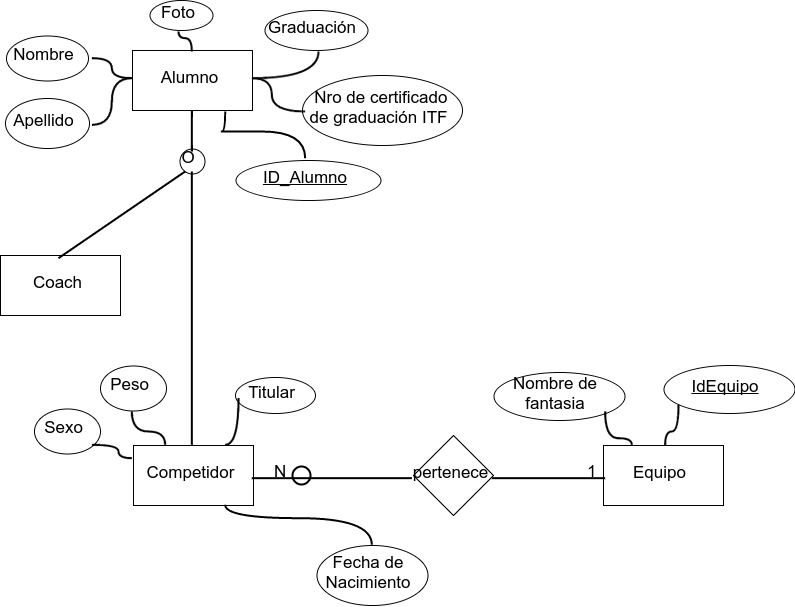
\includegraphics[scale=0.5]{imagenes/AlumnoCompetidor.png}
  \caption{Diagrama centrado en Alumno y Competidor}
\end{figure}

Los alumnos pueden adoptar el rol de un competidor o del coach. A su vez, un competidor puede, o no, formar parte de un equipo
. Se distinguen a los competidores pertenecientes a un equipo por su atributo titular, este indica si se trata de un titular
del equipo o un suplente. En el caso de que no pertenezca a ningún equipo, el atributo titular queda vacío.

\begin{figure}[H]
  \centering
    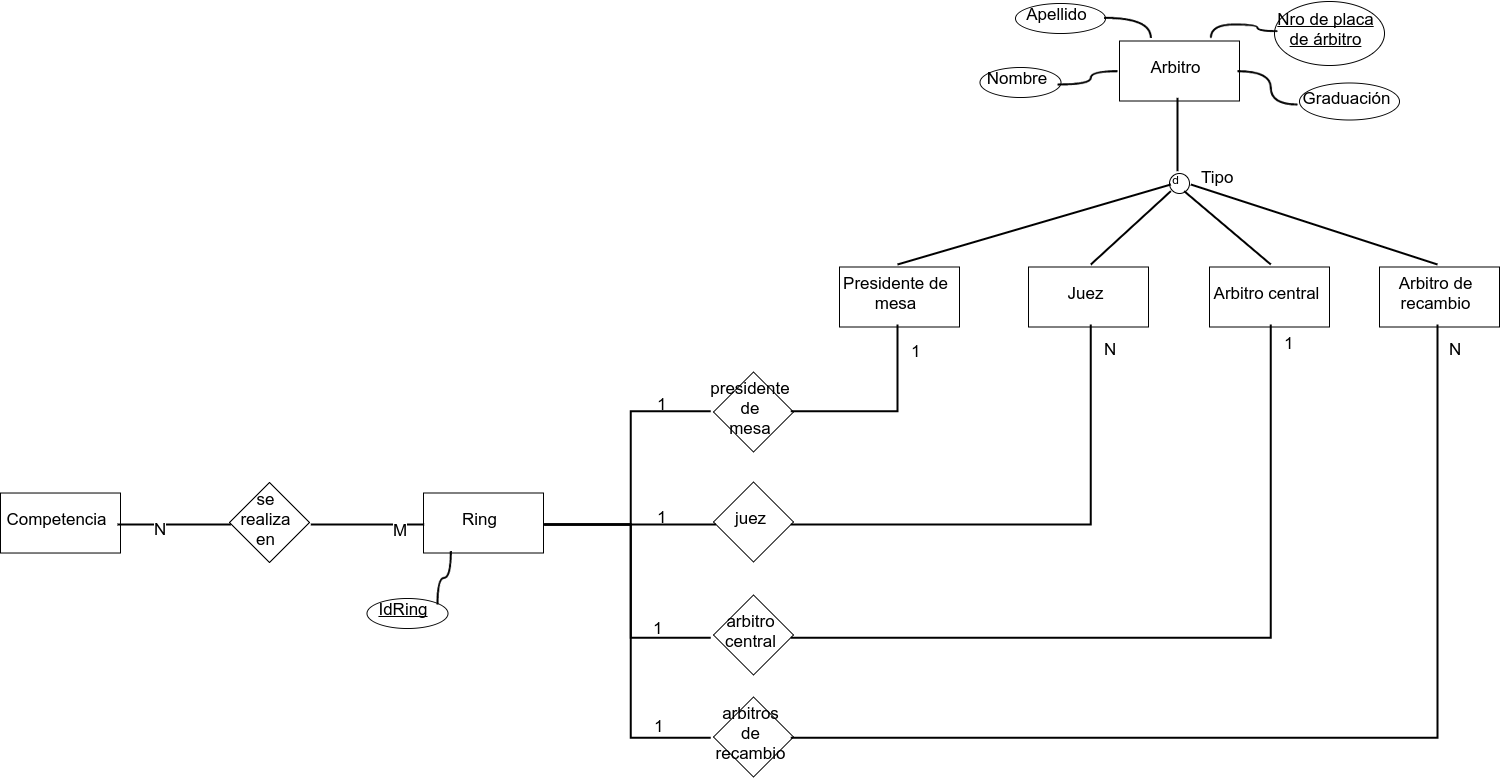
\includegraphics[scale=0.3]{imagenes/ArbitroRing.png}
  \caption{Diagrama centrado en Árbitro y Ring}
\end{figure}

Un árbitro puede ser un presidente de mesa, juez, árbitro central o árbitro de recambio. Cada ring posee un presidente de mesa
y un árbitro central, dependiendo de la competencia varía la cantidad de árbitros correspondientes a los otros tipos.
Un Ring también está asociado a una o más competencias, a su vez para realizar una competencia se podría necesitar de  varios
rings(al menos uno).

\begin{figure}[H]
  \centering
    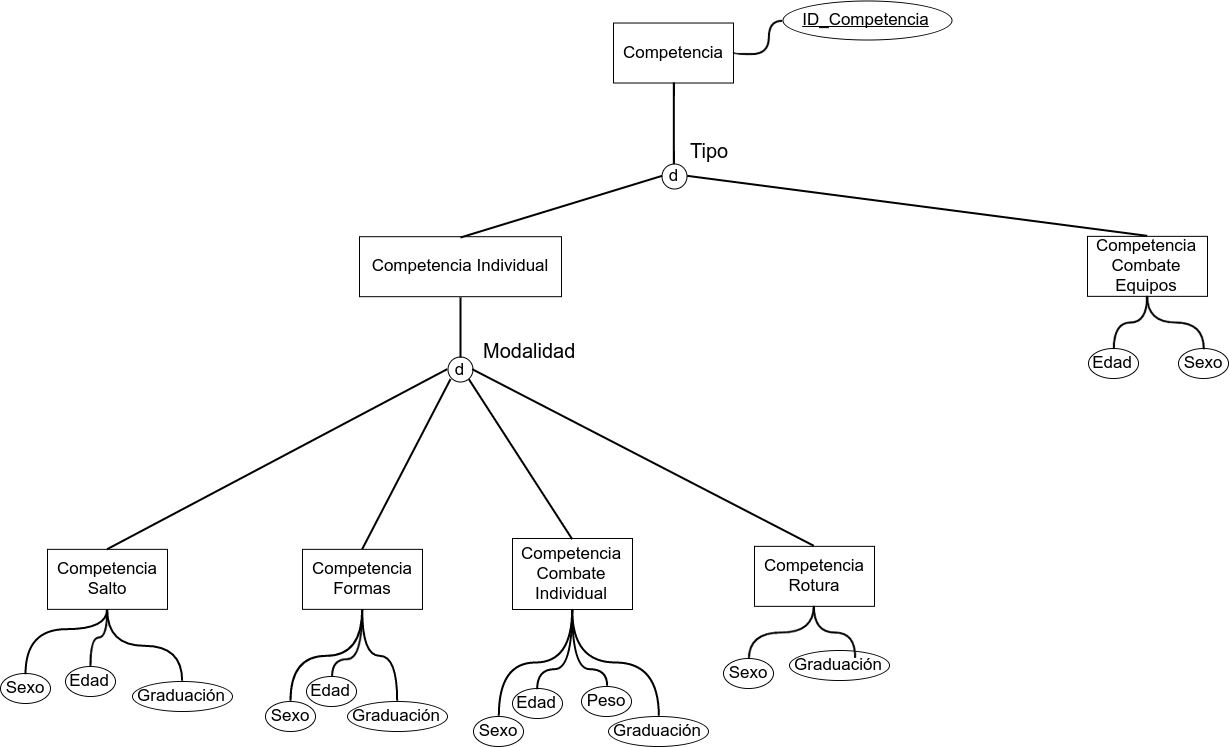
\includegraphics[scale=0.3]{imagenes/Competencia.png}
  \caption{Diagrama centrado en Competencia}
\end{figure}

Las competencias se dividen entre las que son individuales y en las cuales participan equipos. De esta última solo se tiene
 como modalidad a las competencias de combate por equipos, en cambio las competencias individuales poseen 4
 modalidades diferentes. Estas son Salto, Formas, Combate individual, Rotura. Cada una con sus parámetros de participación
 (sexo, edad, etc).

\begin{figure}[H]
  \centering
    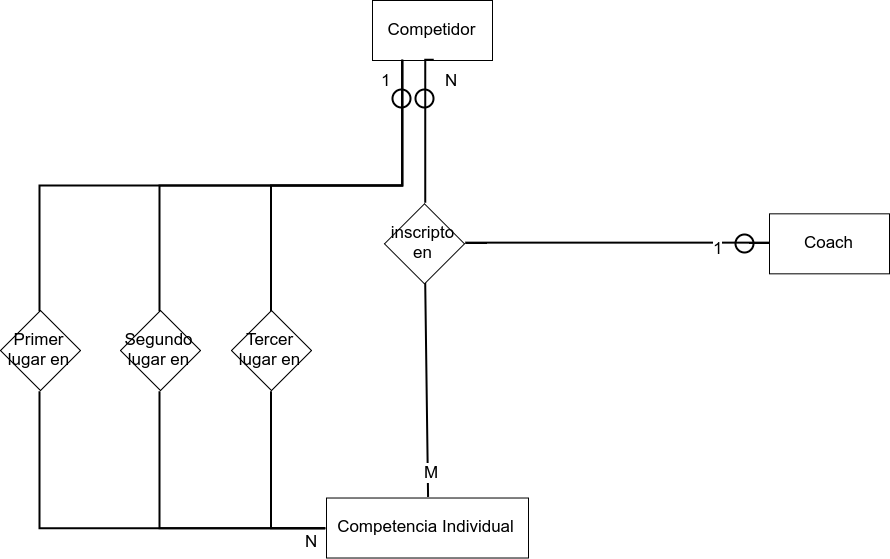
\includegraphics[scale=0.5]{imagenes/CompetidorCompetencia.png}
  \caption{Diagrama centrado en Competidor y Competencia}
\end{figure}

Los competidores se pueden inscribir en una o varias competencias individuales, esto lo hacen supervisado por un coach. A su
vez, el coach puede tener varios de sus competidores inscriptos a una misma competencia. Cada competencia registra a los
competidores que quedaron en los primeros tres lugares.

\begin{figure}[H]
  \centering
    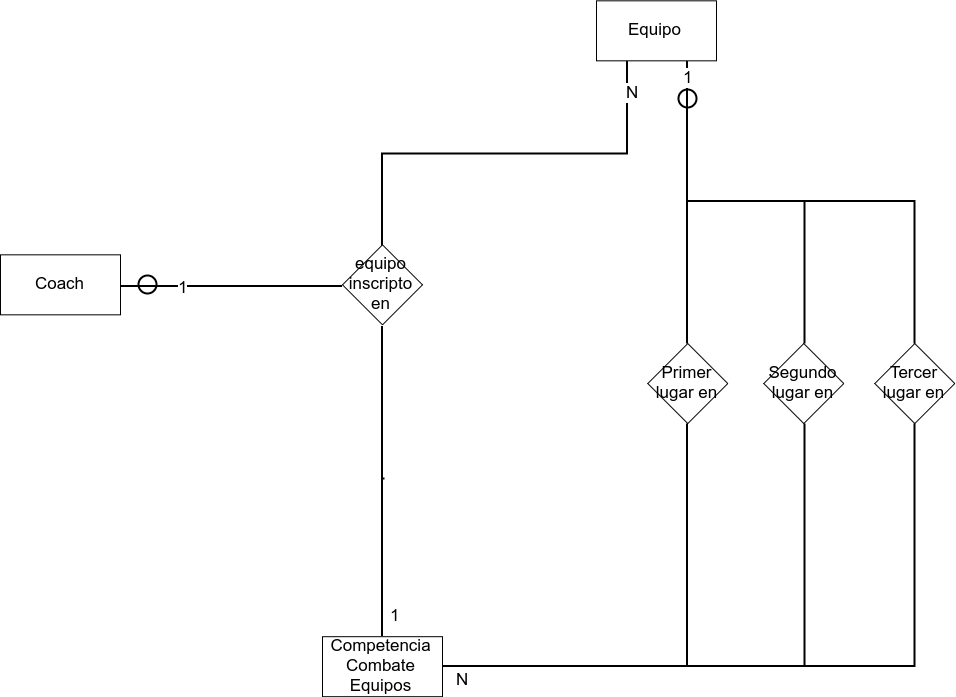
\includegraphics[scale=0.5]{imagenes/EquipoCompetencia.png}
  \caption{Diagrama centrado en Equipo y Competencia}
\end{figure}

Similar que el anterior, pero con las competencias por equipos. La principal diferencia es que en la inscripción, debido a
la cantidad de miembros que deben componer un equipos y la cantidad de competidores que puede supervisar un coach, solamente puede quedar inscripto un equipo por cada
coach en una determinada categoría.

\begin{figure}[H]
  \centering
    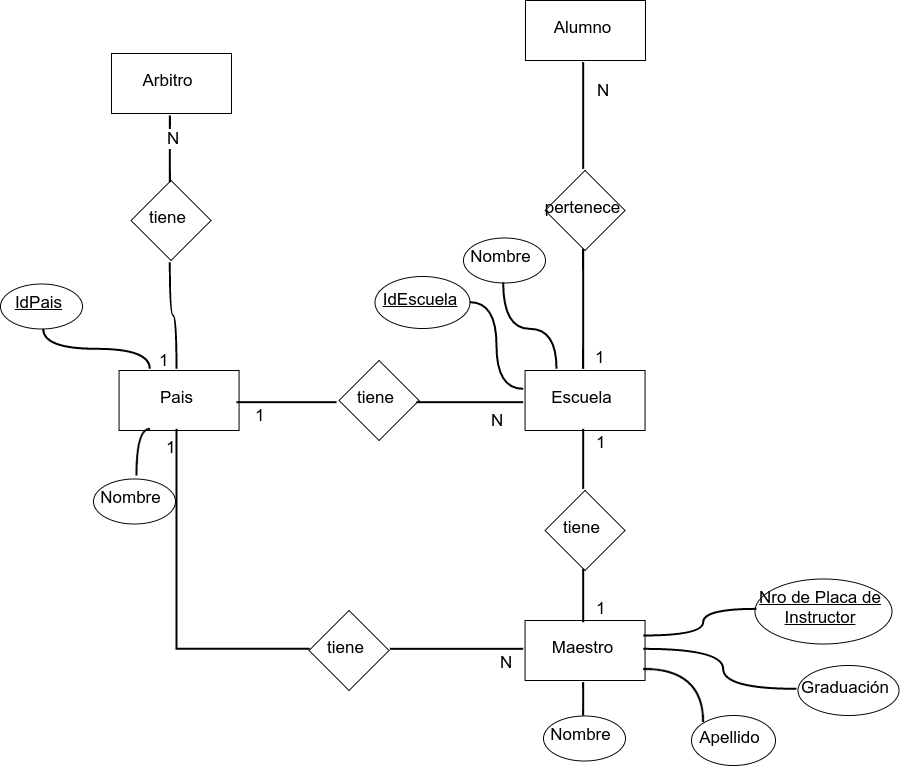
\includegraphics[scale=0.5]{imagenes/EscuelaPais.png}
  \caption{Diagrama centrado en Escuela y País}
\end{figure}

Por último tenemos que tanto Maestros, Árbitros y Escuelas proceden de determinados países. Además cada
escuela posee alumnos y a un maestro que se encarga de la inscripción de los mismos en las competencias.


\newpage
\section{Modelo relacional}
En esta sección se detalla los componentes del modelo relacional creado a partir del modelo entidad relación introducido anteriormente.\\
\\
\textbf{Pais}(\uline{IdPais}, Nombre)\\
PK = \{IdPais\}\\
CK = \{IdPais\}\\
\\
\textbf{Escuela}(\uline{IdEscuela}, Nombre, \dashuline{IdPais})\\
CK = \{IdEscuela\}\\
PK = \{IdEscuela\}\\
FK = \{IdPais\}\\
\\
\textbf{Maestro}(\uline{NroDePlacaDeInstructor}, Nombre, Apellido, Graduación, \dashuline{IdPais}, \dashuline{IdEscuela})\\
CK = \{NroDePlacaDeInstructor\}\\
PK = \{NroDePlacaDeInstructor\}\\
FK = \{IdPais, IdEscuela\}\\
\\
\textbf{Alumno}(\uline{DNI}, Nombre, Apellido, NroCertificadoGraduaciónITF, Graduación, Foto, \dashuline{IdEscuela})\\
CK = \{DNI\}\\
PK = \{DNI\}\\
FK = \{IdEscuela\}\\
\\
\textbf{Equipo}(\uline{IdEquipo}, NombreDeFantasia)\\
PK = \{IdEquipo\}\\
CK = \{IdEquipo\}\\
\\
\textbf{Competidor}(\uline{\dashuline{DNI}}, FechaDeNacimiento, Sexo, Peso, Titular, \dashuline{IdEquipo})\\
CK = \{DNI\}\\
PK = \{DNI\}\\
FK = \{DNI, IdEquipo\}\\
\\
\textbf{Coach}(\uline{\dashuline{DNI}})\\
PK = \{DNI\}\\
CK = \{DNI\}\\
FK = \{DNI\}\\
\\
\textbf{Árbitro}(\uline{NroDePlacaDeÁrbitro}, Nombre, Apellido, Graduación, Tipo, \dashuline{IdPais})\\
CK = \{NroDePlacaDeÁrbitro\}\\
PK = \{NroDePlacaDeÁrbitro\}\\
FK = \{IdPais\}\\
\\
\textbf{Ring}(\uline{IdRing})\\
PK = \{IdRing\}\\
CK = \{IdRing\}\\
\\
\textbf{PresidenteDeMesa}(\dashuline{\uline{NroDePlacaDeÁrbitro}}, \dashuline{IdRing})\\
PK = \{NroDePlacaDeÁrbitro\}\\
CK = \{NroDePlacaDeÁrbitro\}\\
FK = \{NroDePlacaDeÁrbitro, IdRing\}\\
\\
\textbf{Juez}(\dashuline{\uline{NroDePlacaDeÁrbitro}}, \dashuline{IdRing})\\
PK = \{NroDePlacaDeÁrbitro\}\\
CK = \{NroDePlacaDeÁrbitro\}\\
FK = \{NroDePlacaDeÁrbitro, IdRing\}\\
\\
\textbf{ÁrbitroCentral}(\dashuline{\uline{NroDePlacaDeÁrbitro}}, \dashuline{IdRing})\\
PK = \{NroDePlacaDeÁrbitro\}\\
CK = \{NroDePlacaDeÁrbitro\}\\
FK = \{NroDePlacaDeÁrbitro, IdRing\}\\
\\
\textbf{ÁrbitroDeRecambio}(\dashuline{\uline{NroDePlacaDeÁrbitro}}, \dashuline{IdRing})\\
PK = \{NroDePlacaDeÁrbitro\}\\
CK = \{NroDePlacaDeÁrbitro\}\\
FK = \{NroDePlacaDeÁrbitro, IdRing\}\\
\\
\textbf{Competencia}(\uline{IdCompetencia}, Tipo)\\
PK = \{IdCompetencia\}\\
CK = \{IdCompetencia\}\\
\\
\textbf{CompetenciaCombateEquipo}(\dashuline{\uline{IdCompetencia}}, Edad, Sexo, \dashuline{PrimerLugar}, \dashuline{SegundoLugar}, \dashuline{TercerLugar})\\
PK = \{IdCompetencia\}\\
CK = \{IdCompetencia\}\\
FK = \{IdCompetencia, PrimerLugar, SegundoLugar, TercerLugar\}\\
\\
\textbf{CompetenciaIndividual}(\dashuline{\uline{IdCompetencia}}, Modalidad, \dashuline{PrimerLugar}, \dashuline{SegundoLugar}, \dashuline{TercerLugar})\\
PK = \{IdCompetencia\}\\
CK = \{IdCompetencia\}\\
FK = \{IdCompetencia, PrimerLugar, SegundoLugar, TercerLugar\}\\
\\
\textbf{CompetenciaSalto}(\dashuline{\uline{IdCompetencia}}, Sexo, Edad, Graduacion)\\
PK = \{IdCompetencia\}\\
CK = \{IdCompetencia\}\\
FK = \{IdCompetencia\}\\
\\
\textbf{CompetenciaFormas}(\dashuline{\uline{IdCompetencia}}, Sexo, Edad, Graduacion)\\
PK = \{IdCompetencia\}\\
CK = \{IdCompetencia\}\\
FK = \{IdCompetencia\}\\
\\
\textbf{CompetenciaCombateIndividual}(\dashuline{\uline{IdCompetencia}}, Sexo, Edad, Graduacion, Peso)\\
PK = \{IdCompetencia\}\\
CK = \{IdCompetencia\}\\
FK = \{IdCompetencia\}\\
\\
\textbf{CompetenciaRotura}(\dashuline{\uline{IdCompetencia}}, Sexo, Graduacion)\\
PK = \{IdCompetencia\}\\
CK = \{IdCompetencia\}\\
FK = \{IdCompetencia\}\\
\\
\textbf{SeRealizaEn}(\dashuline{\uline{IdCompetencia}}, \dashuline{\uline{IdRing}})\\
PK = \{(IdCompetencia, IdRing)\}\\
CK = \{(IdCompetencia, IdRing)\}\\
FK = \{IdCompetencia, IdRing\}\\
\\
\textbf{InscriptoEn}(\dashuline{\uline{IdCompetencia}}, \dashuline{\uline{IdCompetidor}}, \dashuline{IdCoach})\\
PK = \{(IdCompetencia, IdCompetidor)\}\\
CK = \{(IdCompetencia, IdCompetidor)\}\\
FK = \{IdCompetencia, IdCompetidor, IdCoach\}\\
\\
\textbf{EquipoInscriptoEn}(\dashuline{\uline{IdCompetencia}}, \dashuline{\uline{IdEquipo}}, \dashuline{IdCoach})\\
PK = \{(IdCompetencia, IdEquipo)\}\\
CK = \{(IdCompetencia, IdEquipo)\}\\
FK = \{IdCompetencia, IdEquipo, IdCoach\}\\
\\


\newpage
\section{Restricciones}
En esta sección están especificadas todas las restricciones adicionales del MER y MR introducidos en las secciones anteriores.

\subsection{Restricciónes provenientes del MER:}
\begin{enumerate}
    \item Toda escuela envia un coach por cada cinco competidores inscriptos.
    \item Todos los competidores que pertenecen a un mismo equipo son inscriptos por la misma escuela.
    \item Todo equipo está formado por cinco competidores con el atributo ``Titular'' en true que pertenecen al equipo.
    \item Todo equipo esta formado por al menos tres competidores con el atributo ``Titular'' en false que pertenecen al equipo.
    \item Todo competidor pertenece a un equipo si y solo si el atributo ``Titular'' es distinto de NULL.
    \item Todo competidor inscripto en una competencia es acompañado por un coach enviado por la misma escuela que lo inscribió.
    \item Todo equipo inscripto en una competencia es acompañado por un coach enviado por la misma escuela que inscribió a los competidores del equipo.
    \item Ningún competidor puede ser acompañado en una competencia por un coach que tenga el mismo ``DNI''.
    \item Ningún equipo puede ser acompañado en una competencia por un coach que tenga el mismo ``DNI'' que alguno de sus integrantes.
    \item Todas las competencias que tengan atributo ``Graduación'' deben ser realizadas en rings donde el juez de mesa sea un árbitro con graduación mayor a la de la competencia.
    \item Todas las competencias que tengan atributo ``Graduación'' deben ser realizadas en rings donde todos los jueces sean árbitros con graduación mayor a la de la competencia.
    \item Todas las competencias que tengan atributo ``Graduación'' deben ser realizadas en rings donde el árbitro central sea un árbitro con graduación mayor a la de la competencia.
    \item Todas las competencias que tengan atributo ``Graduación'' deben ser realizadas en rings donde todos los árbitros de recambio sean árbitros con graduación mayor a la de la competencia.
    \item Todo ring tiene al menos tres arbitros de recambio.
    \item Ningún competidor puede estar en más de una de las siguientes relaciones: ``Primer lugar en'', ``Segundo lugar en'', ``Tercer lugar en'' en una misma competencia.
    \item Ningún equipo puede estar en más de una de las siguientes relaciones: ``Primer lugar en'', ``Segundo lugar en'', ``Tercer lugar en'' en una misma competencia.
    \item Todo competidor que está en alguna de las relaciones ``Primer lugar en'', ``Segundo lugar en'' o ``Tercer lugar en'' debe estar inscripto a dicha competencia a la cual pertenece la relación.
    \item Todo Equipo que está en alguna de las relaciones ``Primer lugar en'', ``Segundo lugar en'' o ``Tercer lugar en'' debe estar inscripto y habilitado en dicha competencia a la cual pertenece la relación.
    \item Cada competidor puede estar inscripto en una sola categoria.
\end{enumerate}

\subsection{Restricciones provenientes del MR:}
\begin{itemize}
    \item \textbf{Herencias de Alumno:}
    \begin{itemize}
        \item Competidor.DNI debe estar en Alumno.DNI.
        \item Coach.DNI debe estar en Alumno.DNI.
        \item Alumno.DNI debe estar en Competidor.DNI o (no excluyente) Coach.DNI.
    \end{itemize}
    \item \textbf{Herencias de Competencia:}
    \begin{itemize}
        \item CompetenciaCombateEquipo.IdCompetencia debe estar en Competencia.IdCompetencia
        \item CompetenciaIndividual.IdCompetencia debe estar en Competencia.IdCompetencia
        \item Competencia.IdCompetencia debe estar en CompetenciaCombateEquipo.IdCompetencia o (excluyente) en CompetenciaIndividual.IdCompetencia.
    \end{itemize}
    \item \textbf{Herencias de CompetenciaIndividual:}
    \begin{itemize}
        \item CompetenciaSalto.IdCompetencia debe estar en CompetenciaIndividual.IdCompetencia
        \item CompetenciaFormas.IdCompetencia debe estar en CompetenciaIndividual.IdCompetencia
        \item CompetenciaRotura.IdCompetencia debe estar en CompetenciaIndividual.IdCompetencia
        \item CompetenciaCombateIndividual.IdCompetencia debe estar en CompetenciaIndividual.IdCompetencia
        \item CompetenciaIndividual.IdCompetencia debe estar en CompetenciaSalto.IdCompetencia o (excluyente) en CompetenciaFormas.IdCompetencia o (excluyente) en CompetenciaRotura.IdCompetencia o (excluyente) en CompetenciaCombateIndividual.IdCompetencia.
    \end{itemize}
    \item \textbf{Herencias de Árbitro:}
    \begin{itemize}
        \item PresidenteDeMesa.NroDePlacaDeÁrbitro debe estar en Árbitro.NroDePlacaDeÁrbitro
        \item Juez.NroDePlacaDeÁrbitro debe estar en Árbitro.NroDePlacaDeÁrbitro
        \item ÁrbitroCentral.NroDePlacaDeÁrbitro debe estar en Árbitro.NroDePlacaDeÁrbitro
        \item ÁrbitroDeRecambio.NroDePlacaDeÁrbitro debe estar en Árbitro.NroDePlacaDeÁrbitro
        \item Arbitro.NroDePlacaDeÁrbitro debe estar en PresidenteDeMesa.NroDePlacaDeÁrbitro o (excluyente) en Juez.NroDePlacaDeÁrbitro o (excluyente) ÁrbitroCentral.NroDePlacaDeÁrbitro o (excluyente) en ÁrbitroDeRecambio.NroDePlacaDeÁrbitro.
    \end{itemize}
    \item \textbf{Claves foráneas:}
    \begin{itemize}
        \item Maestro.IdPais debe estar en Pais.IdPais.
        \item Escuela.IdPais debe estar en Pais.IdPais.
        \item Escuela.NroDePlacaDeInstructor debe estar en Maestro.NroDePlacaDeInstructor.
        \item Competidor.IdEscuela debe estar en Escuela.IdEscuela.
        \item Escuela.IdEquipo debe estar en Equipo.IdEquipo o ser NULL.
        \item Coach.IdEscuela debe estar en Coach.IdEscuela.
        \item Árbitro.IdPais debe estar en Pais.IdPais.
        \item CompetenciaIndividual.PrimerLugar debe estar en Competidor.DNI.
        \item CompetenciaIndividual.SegundoLugar debe estar en Competidor.DNI.
        \item CompetenciaIndividual.TercerLugar debe estar en Competidor.DNI.
        \item CompetenciaCombateEquipo.PrimerLugar debe estar en Competidor.DNI.
        \item CompetenciaCombateEquipo.SegundoLugar debe estar en Competidor.DNI.
        \item CompetenciaCombateEquipo.TercerLugar debe estar en Competidor.DNI.
        \item SeRealizaEn.IdCompetencia debe estar en Competencia.IdCompetencia.
        \item SeRealizaEn.IdRing debe estar en Ring.IdRing.
        \item InscriptoEn.IdCompetencia debe estar en Competencia.IdCompetencia.
        \item InscriptoEn.IdCompetidor debe estar en Competidor.DNI.
        \item InscriptoEn.IdCoach debe estar en Coach.DNI.
        \item InscriptoEn.IdCompetencia debe estar en Competencia.IdCompetencia.
        \item InscriptoEn.IdEquipo debe estar en Equipo.IdEquipo.
        \item InscriptoEn.IdCoach debe estar en Coach.DNI.
    \end{itemize}
\end{itemize}


\newpage
\section{Diseño de Base de datos}
\lstinputlisting[language=SQL]{design.sql}

\newpage
\section{Consultas de Base de datos}
\lstinputlisting[language=SQL]{consultas.sql}

\newpage
\section{Triggers y Stored Procedures de Base de datos}
\lstinputlisting[language=SQL]{triggers.sql}

\newpage
\section{Conclusiones}
El diseño y construcción de la base de datos para el Campeonato Mundial de Taekwon-do ITF, resulto en un desafío interesante
para comprobar la efectividad de los modelos y conceptos aprendidos en la materia.
 A lo largo del trabajo práctico nos vimos forzados a repensar varias veces algunas de las partes de nuestro modelo de entidad relación. Algunas de estas fueron la representación del alumno como
competidor individual y como parte de un equipo, la forma en que se representaban las competencias y su relación tanto con
sus competidores como con los ganadores de los primeros tres puestos y la manera en que se asociaban los distintos tipos de
árbitros con los Rings donde se realizaban las competencias. Todos estos problemas aparecieron durante el armado del diagrama de entidad
relación y, por lo tanto, no se necesito realizar cambios demasiado complicados en la base de datos durante su implementación. El diseño de la base de datos resulto simple gracias al modelo
relacional extraído a partir del MER y, a su vez, las restricciones de los mismos fueron muy útiles
para definir los triggers que se necesitaban para garantizar el correcto manejo de los datos. Podríamos concluir que, a pesar de las dificultades que surgieron,
el modelo de entidad relación simplifica enormemente la implementación de una base de datos y dificulta la aparición de
errores graves de diseño a lo largo de la misma.


\end{document}
